\documentclass[conference]{IEEEtran}

\usepackage{cite}
\usepackage{amsmath}
\usepackage{amssymb}
\usepackage{graphicx}
\usepackage{booktabs}
\usepackage{tabularx}
\usepackage{array}
\usepackage{tikz}
\usetikzlibrary{arrows.meta,positioning,shapes.geometric}
\usepackage{url}

\newcolumntype{Y}{>{\raggedright\arraybackslash}X}
\graphicspath{{figs/}{Paper/figs/}}
\tikzset{
  block/.style={draw, rounded corners, align=center, minimum height=7mm, minimum width=21mm, font=\footnotesize},
  smallblock/.style={draw, rounded corners, align=center, minimum height=6mm, minimum width=17mm, font=\scriptsize},
  flow/.style={-{Latex[length=2mm]}, thick}
}

\begin{document}

\title{A Practical Blockchain Framework for Secure and Transparent Airline Ticketing}

\author{\IEEEauthorblockN{Author Name}
\IEEEauthorblockA{Department or Institution\\
City, Country\\
email@example.com}}

\maketitle

\begin{abstract}
Buying a flight ticket is still often dependent on several disconnected systems: a payment provider, a reservation platform, an airline database, and customer-service processes. When those systems disagree, travelers may face failed ticket issuance, slow refunds, or unclear ownership records. This paper proposes a blockchain framework that makes the ticket lifecycle easier to verify. Each valid ticket is represented by a non-fungible token (NFT), and smart contracts manage issuance, transfer, cancellation, and refund events. Large ticket records are kept in the InterPlanetary File System (IPFS), while their cryptographic fingerprints are stored on-chain. The design also combines decentralized identity (DID), elliptic-curve cryptography (ECC), and zero-knowledge proofs (ZKPs) so that a traveler can prove necessary attributes without unnecessarily disclosing personal information. Finally, ERC-2981 is used to define a transparent royalty rule for permitted resale. The proposed model aims to give airlines and travelers a clearer, more secure, and more auditable way to manage ticket transactions. A working prototype on a local Ethereum network completes the full ticket lifecycle: 110 contract tests pass, static analysis reports no high- or medium-severity finding, and a resale payment is split into airline royalty and seller proceeds with no rounding loss.
\end{abstract}

\begin{IEEEkeywords}
Blockchain, decentralized identity, distributed ledger technology, elliptic-curve cryptography, ERC-2981, IPFS, non-fungible token, public-key cryptography, zero-knowledge proof.
\end{IEEEkeywords}

\section{Introduction}
Airline ticketing looks simple from a passenger's perspective, but its back end is not. A payment can be accepted by one service before a reservation system confirms the seat. Refund decisions can pass through several teams. In addition, a traveler has little visibility into what happens to a ticket after it is issued. Centralized booking systems remain useful, but their separate databases and intermediaries can make failures difficult to diagnose and resolve \cite{shaikh2023}.

Blockchain is worth considering here because it gives approved participants a shared, append-only record. It does not solve every airline problem on its own, and it should not be used to store sensitive passenger details openly. However, when combined with off-chain storage and privacy-preserving credentials, it can make ownership, payment settlement, and cancellation events easier to inspect. Earlier studies address secure ticket-distribution access control \cite{zhang2022} and privacy-aware ticketing \cite{cha2018}. What is still needed is a practical design that brings storage efficiency, identity privacy, and an economically realistic resale process into the same ticket lifecycle.

This paper develops that design. Ethereum smart contracts are responsible for rule enforcement and immutable event logging. Ticket records are held off-chain in IPFS and checked against an on-chain hash \cite{pawar2022}. DID, ECC, and ZKPs help verify identity-related conditions without exposing more information than necessary \cite{rizwan2021,cha2018}. ERC-2981 provides a defined royalty mechanism for authorized secondary sales \cite{fekih2023}. The contributions of the paper are:
\begin{itemize}
    \item NFT-based representation of ticket ownership and lifecycle events;
    \item hybrid on-chain/off-chain storage for scalable, verifiable ticket metadata;
    \item privacy-preserving identity verification using DID, ECC, and ZKPs; and
    \item automated resale royalties that establish a transparent airline revenue stream.
\end{itemize}

\begin{table*}[!t]
\caption{Operational and facility deficiencies in conventional airline payment systems}
\label{tab:challenges}
\centering
\footnotesize
\begin{tabularx}{\textwidth}{YY}
\toprule
\textbf{Operational deficiencies} & \textbf{Facility deficiencies}\\
\midrule
Payment may be reported as successful while ticket issuance fails because of synchronization delays between a payment gateway and reservation system. & Limited real-time integration between payment gateways and airline reservation systems.\\
Verification of banking or card transactions may be delayed during peak demand. & Outdated or insufficient server capacity can slow payment processing.\\
Manual intervention may be required to confirm transactions, delaying customers. & Single points of failure and inadequate redundancy in payment infrastructure.\\
Dependence on third-party payment service providers can delay resolution of failed payments. & Insufficient technical support and escalation agreements for immediate failure resolution.\\
Refunds may be delayed because finance and operations are poorly coordinated. & Weak API connectivity among banks, payment providers, and airline systems.\\
Miscommunication can occur between ticketing agents and payment-verification teams. & Monitoring tools may not identify failed or stalled payments in real time.\\
\bottomrule
\end{tabularx}
\end{table*}

\section{Related Work}
Research on blockchain ticketing has moved beyond the idea of simply putting a booking database on a ledger. Traditional booking systems are generally centralized \cite{shaikh2023}; blockchain proposals instead try to create a record that is shared and difficult to alter after the fact \cite{sahoo2023,aldweesh2023}. This distinction is important for tickets because ownership and transaction history may matter long after the original purchase.

Several technical strands inform the design in this paper. Privacy-preserving ticketing research shows how ZKPs can limit unnecessary identity disclosure \cite{cha2018}. ECC is a practical choice for signing and authentication in constrained blockchain environments \cite{rizwan2021}, while blockchain access-control work demonstrates ways to protect passenger data during ticket distribution \cite{zhang2022}. IPFS can keep large records outside the ledger without losing the ability to check whether they have changed \cite{pawar2022}. Formal analysis of ERC contracts also highlights the need to treat NFT contract logic as security-sensitive software \cite{fekih2023}.

Other application areas provide useful lessons. Blockchain has supported multi-party coordination in tourism \cite{bodkhe2019}, automated ticket-like distribution processes \cite{hire2023}, rights management \cite{guadamuz2021}, voucher systems \cite{hsu2020}, and aviation data sharing \cite{clementi2019}. The proposed framework builds on these separate ideas, but applies them together to the everyday events of issuing, transferring, and cancelling an airline ticket.

\begin{table*}[!t]
\caption{Comparative analysis of related work}
\label{tab:related}
\centering
\footnotesize
\begin{tabularx}{\textwidth}{p{.20\textwidth}Yp{.24\textwidth}p{.22\textwidth}}
\toprule
\textbf{Work} & \textbf{Objective} & \textbf{Approach} & \textbf{Representative technologies}\\
\midrule
Airline booking system \cite{shaikh2023} & Store and retrieve travel information in a reservation system. & Centralized computerized booking application. & CSS, HTML, PHP\\
Air-ticket distribution access control \cite{zhang2022} & Protect passenger data and ticket-distribution assets. & Blockchain-powered access-control framework. & Hyperledger Fabric, SM2\\
Privacy-preserving ticketing \cite{cha2018} & Protect ticket-holder privacy in blockchain ticketing. & Non-interactive ZKP-based ticketing. & NIZK, blockchain\\
BloHosT \cite{bodkhe2019} & Coordinate stakeholders in tourism and hospitality. & Collaborative blockchain framework with a shared wallet identity. & Blockchain, Proof of Collaboration, ZKP\\
Decentralized lottery \cite{hire2023} & Automate ticket sale and winner selection. & Smart contract enforces lottery rules and a verifiable outcome. & Ethereum, Solidity, smart contracts\\
Airline ticketing with blockchain \cite{sahoo2023} & Improve provenance, immutability, and transparency. & Blockchain-based management of centralized airline ticketing limitations. & DLT, encryption, digital signatures\\
BlockTicket \cite{aldweesh2023} & Remove intermediaries and reduce data-breach risk in e-ticketing. & Smart-contract e-ticketing framework. & P2P, blockchain, hashing\\
\bottomrule
\end{tabularx}
\end{table*}

\section{Architecture and Implementation}
Figure~\ref{fig:lifecycle} summarizes the ticket lifecycle. A traveler sends a purchase request and payment to a smart contract. If the contract accepts the transaction, it creates a unique ERC-721 NFT and assigns it to the traveler's wallet. The contract also records how the payment should be settled. If the traveler cancels, the same contract checks ownership and the relevant fare rules before it revokes the ticket and processes the refund. If the airline permits a later transfer, ERC-2981 can reserve a royalty share for the airline.

\begin{figure}[!t]
\centering
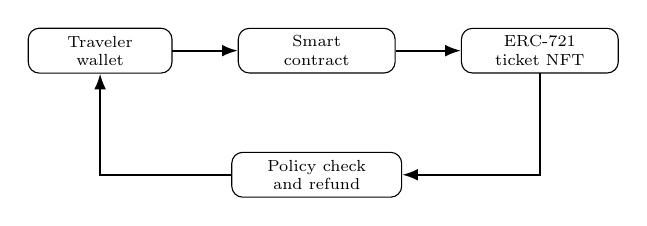
\begin{tikzpicture}[node distance=8mm and 10mm, scale=.83, transform shape]
\node[smallblock, minimum width=22mm] (traveler) {Traveler\\wallet};
\node[smallblock, minimum width=24mm, right=of traveler] (contract) {Smart\\contract};
\node[smallblock, minimum width=24mm, right=of contract] (nft) {ERC-721\\ticket NFT};
\node[smallblock, minimum width=26mm, below=12mm of contract] (refund) {Policy check\\and refund};
\draw[flow] (traveler) -- (contract);
\draw[flow] (contract) -- (nft);
\draw[flow] (nft.south) |- (refund.east);
\draw[flow] (refund.west) -| (traveler.south);
\end{tikzpicture}
\caption{Decentralized air-ticket purchase and cancellation process.}
\label{fig:lifecycle}
\end{figure}

The model is deliberately not tied to one country or one group of carriers. Airlines may run validator nodes in a permissioned consortium, or they may connect selected processes to a public blockchain. The appropriate choice depends on regulation, data-governance requirements, and the commercial relationship among airlines. A common ERC-721 interface makes it possible to verify tickets across participating carriers without forcing them to give up control of their own operations.

Figure~\ref{fig:architecture} gives a high-level view of the proposed architecture. The web application is the main interaction point for travelers and airline staff. Wallets sign requests, while smart contracts maintain the authoritative lifecycle state for flights, tickets, payments, refunds, and permitted resale. IPFS holds ticket metadata outside the blockchain; the ticket contract stores the corresponding CID so that a retrieved record can be checked for integrity.

\begin{figure*}[!t]
\centering
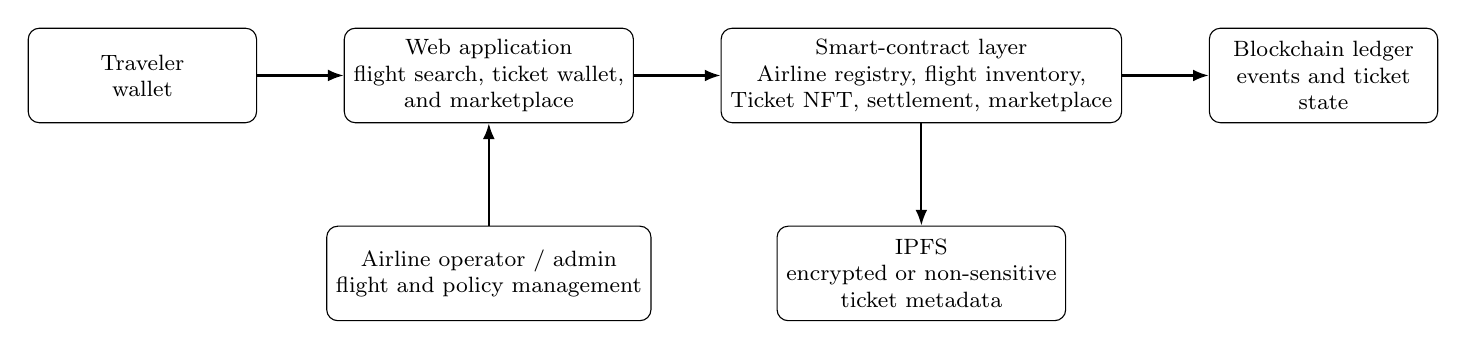
\begin{tikzpicture}[node distance=8mm and 11mm]
\node[block, minimum width=29mm, minimum height=12mm] (traveler) {Traveler\\wallet};
\node[block, minimum width=31mm, minimum height=12mm, right=of traveler] (dapp) {Web application\\flight search, ticket wallet,\\and marketplace};
\node[block, minimum width=39mm, minimum height=12mm, right=of dapp] (contracts) {Smart-contract layer\\Airline registry, flight inventory,\\Ticket NFT, settlement, marketplace};
\node[block, minimum width=29mm, minimum height=12mm, right=of contracts] (ledger) {Blockchain ledger\\events and ticket\\state};
\node[block, minimum width=31mm, minimum height=12mm, below=13mm of dapp] (operator) {Airline operator / admin\\flight and policy management};
\node[block, minimum width=31mm, minimum height=12mm, below=13mm of contracts] (ipfs) {IPFS\\encrypted or non-sensitive\\ticket metadata};
\draw[flow] (traveler) -- (dapp);
\draw[flow] (dapp) -- (contracts);
\draw[flow] (contracts) -- (ledger);
\draw[flow] (operator) -- (dapp);
\draw[flow] (contracts) -- (ipfs);
\end{tikzpicture}
\caption{High-level architecture of the proposed blockchain airline-ticketing framework.}
\label{fig:architecture}
\end{figure*}

\section{Recommended Framework}
Figure~\ref{fig:workflow} shows how the main components work together. The traveler first connects a wallet to a DID. The DID can carry W3C-compatible verifiable credentials that are signed using ECC. Once a flight is selected and payment is submitted, the smart contract applies the ticketing rules. The detailed ticket record is then stored in IPFS, and its content identifier (CID) is written to the NFT's \texttt{tokenURI}. Whenever the record is retrieved, its CID can be compared with the on-chain value to detect alteration.

\begin{figure}[!t]
\centering
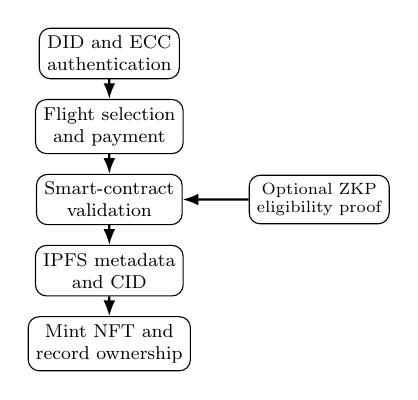
\begin{tikzpicture}[node distance=3mm, scale=.84, transform shape]
\node[block] (did) {DID and ECC\\authentication};
\node[block, below=of did] (select) {Flight selection\\and payment};
\node[block, below=of select] (verify) {Smart-contract\\validation};
\node[block, below=of verify] (ipfs) {IPFS metadata\\and CID};
\node[block, below=of ipfs] (nft) {Mint NFT and\\record ownership};
\node[smallblock, right=10mm of verify] (zkp) {Optional ZKP\\eligibility proof};
\draw[flow] (did) -- (select);
\draw[flow] (select) -- (verify);
\draw[flow] (verify) -- (ipfs);
\draw[flow] (ipfs) -- (nft);
\draw[flow] (zkp) -- (verify);
\end{tikzpicture}
\caption{Workflow of the proposed system.}
\label{fig:workflow}
\end{figure}

\subsection{Ticket Purchase Framework}
The purchase stage begins with a wallet and DID that together provide a verifiable, user-controlled identity. When the airline issues a ticket, it mints an NFT that points to metadata containing flight details, date, seat information, and a hashed passenger reference. The information itself is not placed directly on the blockchain. It stays in IPFS or, where policy requires, in an airline-managed system. The chain holds the CID needed to confirm the record's integrity.

An approved marketplace can then use the NFT as the ticket's ownership record. After a buyer pays, the smart contract transfers the NFT and releases the funds according to the airline's settlement rules. A ZKP can be used when the traveler must prove an attribute---for example, that a required travel credential is valid---without revealing the credential itself. For a permitted resale, the contract applies the ERC-2981 royalty rule automatically.

This division of responsibility keeps the blockchain focused on facts that need strong auditability: ownership changes, settlement outcomes, and IPFS references. It avoids the cost and privacy concerns of writing full ticket records to a public ledger, while still allowing authorized parties to verify key events.

\subsection{Ticket Cancellation Framework}
Cancellation uses the same ownership record rather than a separate manual reconciliation process. When a traveler submits a cancellation request, the contract confirms that the requesting wallet owns the ticket and then checks the relevant timing and fare rules. One possible time-sensitive refund policy is
\begin{equation}
R = P\left(1-c^{t}\right),
\label{eq:refund}
\end{equation}
where $R$ is the refund value, $P$ is the original ticket price, $c$ is a penalty factor defined by the fare policy, and $t$ is the time remaining before departure in a chosen unit. This is an illustrative rule, not a universal fare formula. A real deployment must implement the airline's published conditions and applicable consumer-protection requirements.

Once the checks pass, the contract burns the NFT or transfers it to a controlled null address, adds a revocation event to the ledger, and sends the calculated refund to the traveler's wallet. If airline policy permits, the airline may then release the seat for sale again. Each step remains visible in the event history, which reduces the ambiguity that often appears in a manual cancellation workflow.

\begin{figure}[!t]
\centering
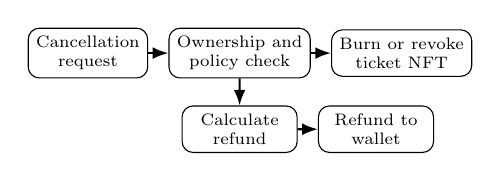
\begin{tikzpicture}[node distance=4mm and 3mm, scale=.86, transform shape]
\node[smallblock] (request) {Cancellation\\request};
\node[smallblock, right=of request] (check) {Ownership and\\policy check};
\node[smallblock, right=of check] (revoke) {Burn or revoke\\ticket NFT};
\node[smallblock, below=of check] (calc) {Calculate\\refund};
\node[smallblock, right=of calc] (pay) {Refund to\\wallet};
\draw[flow] (request) -- (check);
\draw[flow] (check) -- (revoke);
\draw[flow] (check) -- (calc);
\draw[flow] (calc) -- (pay);
\end{tikzpicture}
\caption{Proposed airline-ticket cancellation flow.}
\label{fig:cancellation}
\end{figure}

\section{Testing and Evaluation}
The framework was implemented as a working prototype so that the design rules above could be checked in practice rather than only on paper. The prototype uses Solidity 0.8.28 with OpenZeppelin 5.6.1, a local Hardhat development chain (chainId 31337), ethers v6, and a plain HTML/JavaScript front end that talks to the contracts through an injected wallet. Ticket metadata is uploaded through a small protected endpoint; when no storage provider is configured, the system generates a deterministic mock content identifier and labels the record accordingly. All data is fictional and every value transfer uses test ether.

\subsection{Contract Testing and Static Analysis}
The five contracts and the protected upload endpoint are covered by 110 automated tests, distributed as 15 registry, 11 inventory, 12 ticket-NFT, 31 settlement, 33 marketplace, and 8 upload-endpoint checks. Every public state-changing function is exercised on its success path and on its failure path, including role violations, invalid or out-of-range arguments, pause states, terminal ticket states, refund-deadline boundaries, resale price and expiry caps, cross-airline withdrawal attempts, and repeated cancellation of a ticket that has already reached its terminal state. Table~\ref{tab:verification} summarizes the verification results.

\begin{table}[!t]
\caption{Verification results of the implemented prototype}
\label{tab:verification}
\centering
\footnotesize
\begin{tabularx}{\columnwidth}{p{.33\columnwidth}Y}
\toprule
\textbf{Check} & \textbf{Result}\\
\midrule
Unit tests (6 suites) & 110/110 pass, including failure paths for every public write\\
Static analysis (Slither 0.11.5) & 0 high and 0 medium findings; 19 low/informational items documented\\
Contract linting (Solhint) & 0 errors\\
Credential scan & No secrets in tracked source\\
Scripted demo scenario & 7/7 steps pass, non-zero exit on failure\\
Browser end-to-end (Playwright) & 21/21 tests pass, no uncaught page errors\\
\bottomrule
\end{tabularx}
\end{table}

Rejected operations are checked against their named custom errors rather than against a generic failure. A second cancellation of a ticket that is already cancelled reverts with \texttt{NotIssued\_\_state}; a cancellation, a resale listing, or a new booking after departure reverts with \texttt{FlightDeparted\_\_id}; a listing above the resale cap reverts with \texttt{ResaleCapExceeded\_\_price}; an expiry beyond the check-in boundary reverts with \texttt{ExpiryPastCheckin\_\_expiresAt}; an attempt to list a ticket the caller does not own reverts with \texttt{NotTicketOwner\_\_caller}; and a wallet that has not been approved cannot create a flight (\texttt{NotApproved\_\_wallet}). Unit tests assert these rejections directly, and the scripted demonstration repeats the departure-related ones against the same chain state it uses for the happy path, so the evaluation covers both the success and the failure side of every public operation.

Static analysis was run with Slither 0.11.5 against the same compiler version. No high- or medium-severity issue remains. The reentrancy reports on the payout paths were resolved by ordering state updates before external transfers, the uninitialized-value report was resolved by initializing the affected return variable, and the one suppressed finding (arbitrary ether send) concerns an administrator-gated pull withdrawal that can only move funds already credited to per-airline balances. The nineteen remaining findings are informational --- block-timestamp dependence, benign reentrancy annotations, low-level calls used with explicit recipients, and event-indexing suggestions --- and each one is recorded together with its disposition. The full report is archived with the source, and the analysis is rerun as part of the release gate after every contract change, so a regression that reintroduced a high- or medium-severity finding would fail the gate rather than surface during a review.

Beyond the static tooling, the test suite pins down the runtime security posture. The platform pause blocks flight creation, publishing, booking, listing, resale, and transfers while leaving cancellation, boarding, and reads available so that an active ticket can always be resolved; a deactivated operator cannot create new flights while tickets already issued under it remain valid; withdrawal pays each airline only its own credit less the refund reserve; and no administrative function can move a ticket, a seat, or another account's balance. Each of these properties is asserted as a test rather than left to review, which is why the security argument for the prototype rests on executed checks instead of on the code's appearance.

\subsection{Scenario Evaluation}
A scripted evaluator performs the complete demonstration from a fresh chain. An administrator approves an airline operator wallet; the operator publishes a five-seat flight with a 0.1~ETH fare, an 80\% refund policy, and a 5\% resale royalty; a traveler buys seat \texttt{S-1} and receives an ERC-721 ticket; the public verifier reports the ticket through exactly seven non-identity fields; the ticket is listed at 0.11~ETH (within the 120\% cap) and bought by a third wallet, which pays the airline 0.0055~ETH and the seller 0.1045~ETH --- an exact partition of the payment with no rounding loss beyond the documented integer-division rule; a second ticket is cancelled for a 0.08~ETH refund that retains 0.02~ETH, with the seat returning to inventory; and after the flight is marked departed, cancellation, resale, and new bookings all revert with a departure error. All seven steps pass, and the evaluator records the transaction hash of each lifecycle transaction, so every figure quoted here can be traced to an individual transaction on the local chain.

Table~\ref{tab:gas} reports the gas consumed by the main lifecycle transactions on the local EVM. Ticket issuance is the most expensive operation because a single transaction mints the NFT, reserves the seat, and updates settlement and escrow accounting, while marking a flight departed is an order of magnitude cheaper. The figures are indicative rather than definitive: they were measured on an unloaded local node with the default (unoptimized) compiler settings. Table~\ref{tab:demo} lists the observed outcome of each of the seven steps, in the order the evaluator executes them.

The evaluator asserts those outcomes rather than merely printing them. Around every transaction it compares the settlement balance, the per-airline credit, and the refund reserve against independently computed expectations; after a resale it checks that the marketplace contract retains no ether, that the airline received exactly the royalty, and that the seller received exactly the remainder; after a cancellation it checks that the escrow released precisely one ticket's reserve, that the airline's credit was debited by the refund, and that the vacated seat reappeared in the inventory pool; and it confirms that a terminal state cannot be left again. Any mismatch aborts the run with a non-zero exit code, so a green result means the accounting reconciled to the wei at every step rather than that the transactions merely succeeded.

\begin{table}[!t]
\caption{Gas used by the main lifecycle transactions (local EVM, optimizer disabled)}
\label{tab:gas}
\centering
\footnotesize
\begin{tabularx}{\columnwidth}{Yrl}
\toprule
\textbf{Operation} & \textbf{Gas} & \textbf{Tx (prefix)}\\
\midrule
Purchase (mint + reserve + accounting) & 386\,325 & \texttt{0xce82$\cdot\cdot$}\\
List ticket for resale & 310\,302 & \texttt{0xa44f$\cdot\cdot$}\\
Buy listing (royalty + proceeds split) & 185\,674 & \texttt{0x6292$\cdot\cdot$}\\
Cancel ticket (refund + seat return) & 196\,265 & \texttt{0x2bbf$\cdot\cdot$}\\
Mark flight departed & 33\,049 & \texttt{0x2075$\cdot\cdot$}\\
\bottomrule
\end{tabularx}
\end{table}

\begin{table}[!t]
\caption{Observed outcome of each demonstration step}
\label{tab:demo}
\centering
\footnotesize
\begin{tabularx}{\columnwidth}{p{.07\columnwidth}Y}
\toprule
\textbf{\#} & \textbf{Observation}\\
\midrule
1 & Airline wallet approved; role and approval flag set\\
2 & \texttt{R1-DEMO-001} published: 5 seats, 0.1~ETH fare, 80\% refund, 5\% royalty\\
3 & Ticket 1 issued on seat \texttt{S-1}; settlement holds 0.1~ETH with a 0.08~ETH reserve\\
4 & Verifier reports 7 non-identity fields, state \texttt{Issued}, preview 0.08/0.02~ETH\\
5 & 0.11~ETH splits into 0.0055~ETH royalty and 0.1045~ETH proceeds, atomically\\
6 & Ticket 2 \texttt{Cancelled}: 0.08~ETH refunded, 0.02~ETH retained, seat returned\\
7 & \texttt{FlightDeparted\_\_id} rejects cancellation, resale, and a new booking\\
\bottomrule
\end{tabularx}
\end{table}

The front end is covered by 21 automated browser tests covering public verification without a wallet, the full purchase-to-resale-to-cancellation journey, administrative role gating, and responsive and accessibility checks at a 375~px viewport, with screenshots captured at each stage. Two implementation lessons are worth recording. First, keeping the marketplace as the only authority over resale arithmetic meant the display-only royalty view and the settlement path could not drift apart: both read the same stored basis points, and the evaluator checks the split against an independently computed expectation. Second, deriving the administrative audit feed from a bounded scan of contract events avoided deploying an indexer while still attributing every action to a transaction hash; that trade-off is acceptable for a prototype with a bounded history window but not for an archive that must grow indefinitely. The evaluation confirms the success metrics of the prototype: the scripted flows complete on the local network, every public write has passing success and failure-path tests, no credentials appear in tracked client code, no unresolved high-severity finding remains, a verifier can identify a ticket's state without access to personal data, and a resale event accounts for 100\% of the payment as seller proceeds plus airline royalty.

\subsection{Reproducibility and Evidence}
All numbers reported in this section come from the repository's own gates, which can be rerun from a clean checkout. \texttt{npm test} boots a local chain and runs the unit suites; \texttt{npm run eval} redeploys the stack and replays the seven-step demonstration, printing one pass/fail line per step, the gas used and the transaction hash of each lifecycle transaction, and a JSON summary that can be archived with the submission; \texttt{npm run test:e2e} starts a node, a static file server, and the browser suite; and Slither, Solhint, and the credential scan run as separate steps. The static-analysis report, the evaluator summary, and the screenshots produced by the browser suite are stored alongside the source, so the evaluation can be repeated rather than taken on trust.

The browser suite supplies the remaining evidence. It verifies that the public pages load with no wallet attached, walks the complete journey from booking to cancellation, checks the administrative role gating, confirms that no page raises an uncaught console error, and loads every page at a 375\,px viewport to assert that nothing scrolls horizontally and that each control carries an accessible label. The interface checks are part of the evidence rather than decoration: status messages must be announced through a live region, a page refresh must not discard an operator's in-progress edit, and a rejected transaction must be reported as a sentence rather than as raw custom-error data. Figure~\ref{fig:screenshots} shows three stages of the demonstration as captured by that suite: the booking confirmation after the mint transaction settles, the public verification page that reports the ticket without any personal data, and the marketplace after the resale has distributed the royalty and the proceeds.

\begin{figure*}[!t]
\centering
\footnotesize
\begin{minipage}[b]{0.31\textwidth}
\centering
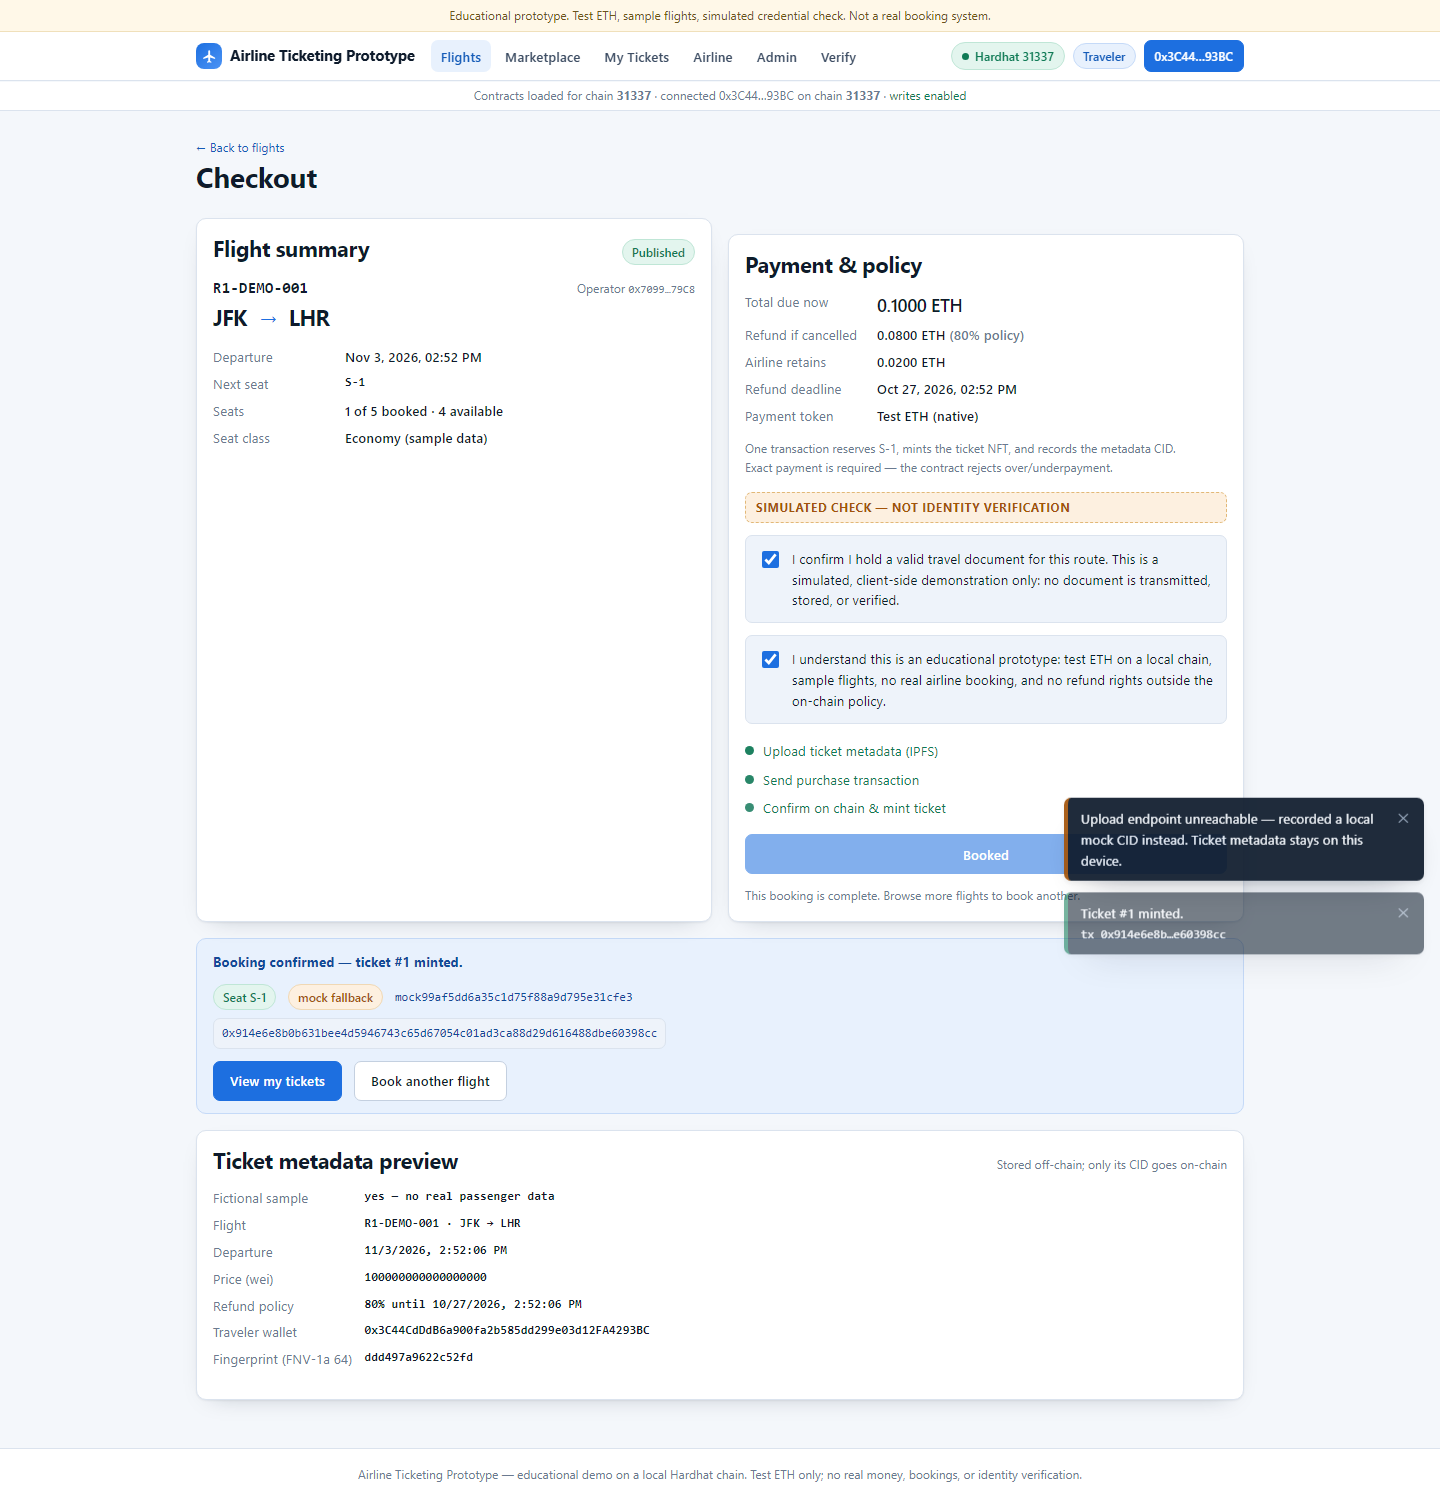
\includegraphics[width=\linewidth]{booking-confirmed}\\[-1pt]
\textit{(a) Booking confirmed}
\end{minipage}\hfill
\begin{minipage}[b]{0.31\textwidth}
\centering
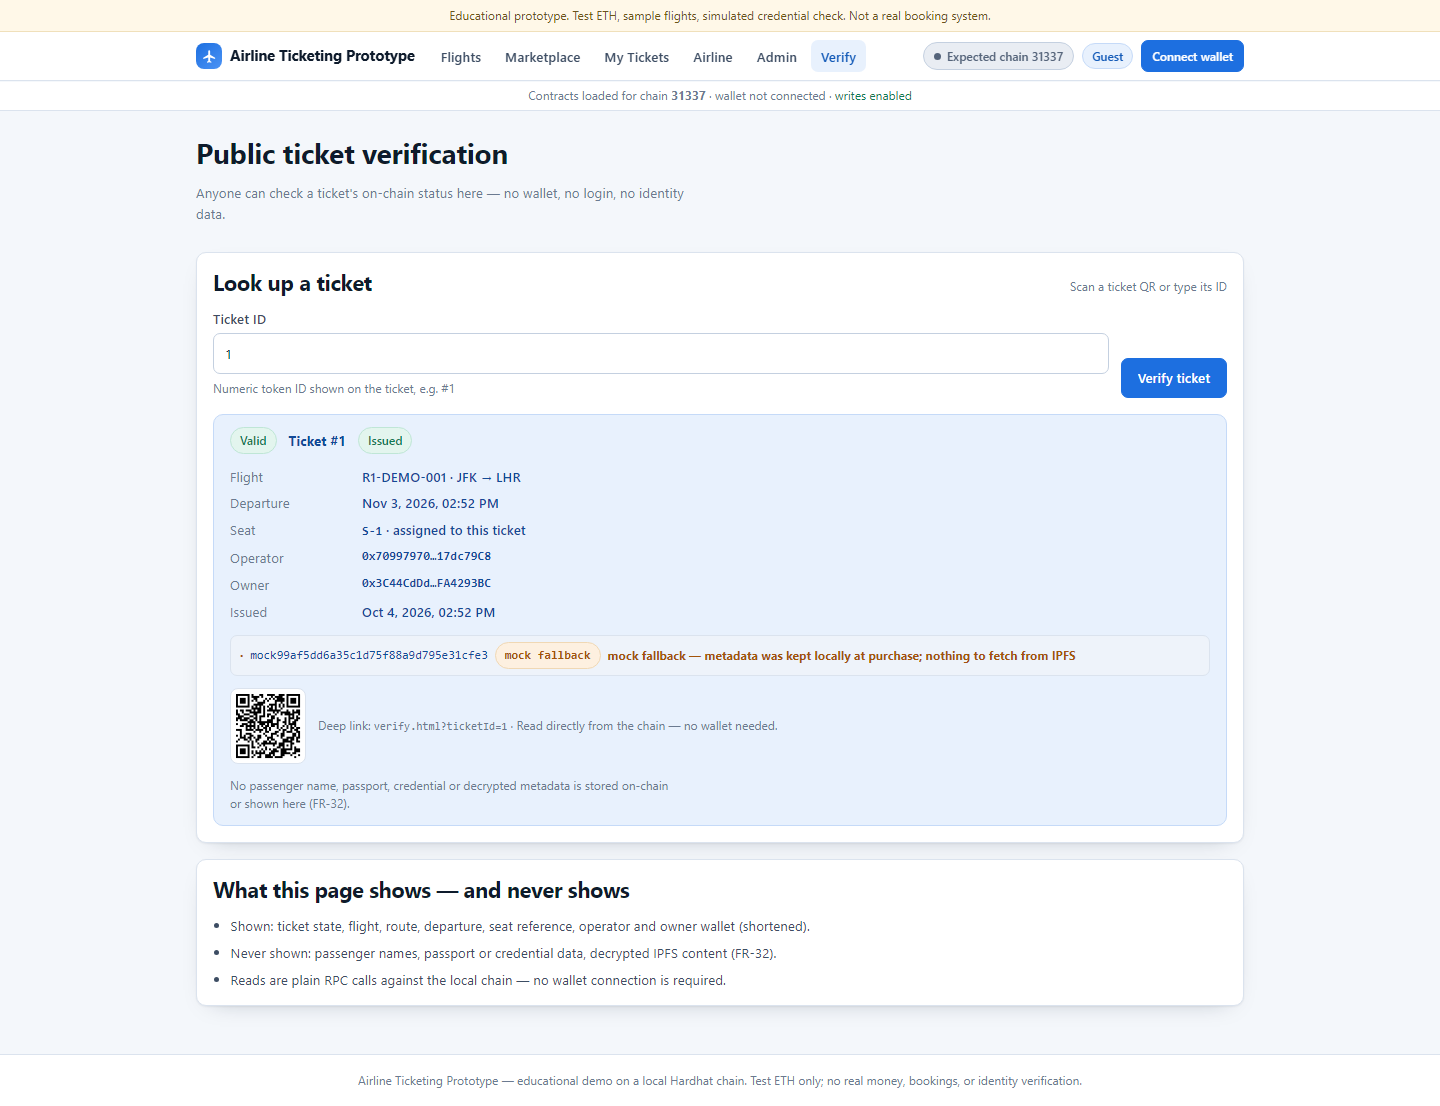
\includegraphics[width=\linewidth]{verify-issued}\\[-1pt]
\textit{(b) Public verification}
\end{minipage}\hfill
\begin{minipage}[b]{0.31\textwidth}
\centering
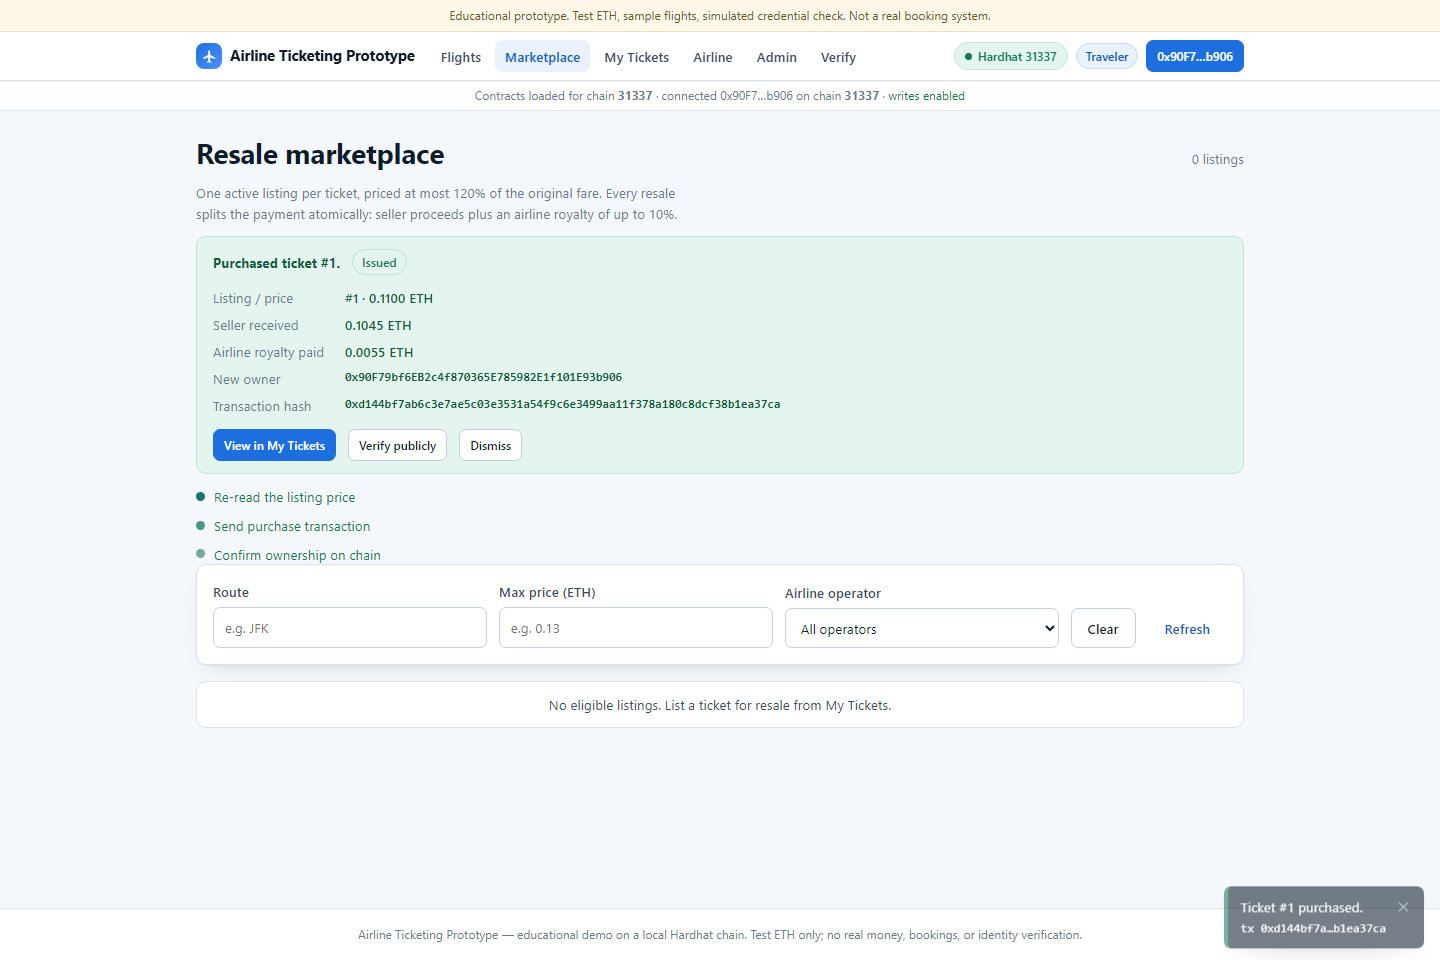
\includegraphics[width=\linewidth]{resale-settled}\\[-1pt]
\textit{(c) Resale settled}
\end{minipage}
\caption{Prototype evidence captured by the browser test suite: (a) the ticket is minted after payment is confirmed, (b) the public verifier reports the issued state from seven non-identity fields, and (c) the completed resale pays the airline royalty and the seller proceeds in a single transaction.}
\label{fig:screenshots}
\end{figure*}

\subsection{Limitations}
Relative to the systems compared in Table~\ref{tab:related}, the prototype contributes an executable combination of ideas that earlier work usually proposes separately: access-controlled issuance, off-chain metadata with an on-chain fingerprint, a verifier surface that exposes no personal data, and a royalty split enforced inside the settlement transaction rather than by convention. The evaluation shows that these rules can coexist in one ticket lifecycle without an indexer or a trusted off-chain component in the settlement path.

The prototype runs on a single local node with test ether, so no conclusion can yet be drawn about throughput, latency, or cost under real demand, and the gas figures are not comparable to a production network. There is no integration with a real reservation or payment system, identity validation is simulated rather than backed by issued credentials, and metadata storage falls back to a labeled mock identifier when no IPFS provider is configured. These constraints bound the evaluation to functional correctness, accounting exactness, and security posture.

The evaluation is therefore functional rather than statistical. It shows that the rules hold when they are exercised in sequence on one deterministic chain, but a single run says nothing about concurrent transactions, and the measurements come from a simulated EVM without the optimizer a production deployment would use. The accounts, flight, and fares are fixed fixtures, so the results characterize the implementation of the rules rather than any particular route, airline, or booking volume.

\section{Conclusion and Future Work}
This paper outlines a practical way to make airline ticketing more transparent without putting sensitive ticket records directly on a blockchain. NFTs provide a clear representation of ticket ownership. Smart contracts record and enforce the events that matter most: issue, transfer, cancellation, and refund. IPFS keeps detailed metadata scalable, while DID, ECC, and ZKPs support a more privacy-conscious identity process. ERC-2981 adds a visible rule for airline participation in authorized resale.

The framework is implemented as a working prototype on a local Ethereum network, where the scripted demonstration completes the full lifecycle and the resale payment settles as an exact royalty-plus-proceeds split. Validation in a real operating environment is still required. Future work should connect the prototype to airline and reservation-system partners, measure performance under realistic demand, examine interoperability between chains and existing booking platforms, and optimize ZKP verification. It should also study the legal, consumer-protection, and economic consequences of a royalty-enabled ticket resale market.

\begin{thebibliography}{00}
\bibitem{shaikh2023} M. Shaikh and R. Borate, ``Airline Booking System,'' \emph{Technoarete Transactions on Advances in Computer Applications}, vol. 2, no. 1, pp. 12--18, 2023.
\bibitem{pawar2022} M. K. Pawar \emph{et al.}, ``Performance Analysis of E-Certificate Generation and Verification Using Blockchain and IPFS,'' in \emph{Proc. Int. Conf. Inventive Computation Technologies (ICICT)}, 2022, pp. 345--350, doi: 10.1109/ICICT54344.2022.9850830.
\bibitem{rizwan2021} M. Rizwan, M. N. Sohail, A. Asheralieva, A. Anjum, and P. Angin, ``SAID: ECC-Based Secure Authentication and Incentive Distribution Mechanism for Blockchain-Enabled Data Sharing System,'' in \emph{Proc. IEEE Int. Conf. Blockchain}, 2021, pp. 530--537, doi: 10.1109/Blockchain53845.2021.00080.
\bibitem{fekih2023} R. B. Fekih, M. Lahami, M. Jmaiel, and S. Bradai, ``Formal Modeling and Verification of ERC Smart Contracts: Application to NFT,'' in \emph{Proc. IEEE Symp. Computers and Communications (ISCC)}, 2023, pp. 556--561, doi: 10.1109/ISCC58397.2023.10218105.
\bibitem{zhang2022} L. Zhang, T. Wang, and Z. Wu, ``Access Control Method for Air Ticket Distribution System Based on Blockchain,'' in \emph{Proc. IEEE Intl. Conf. Parallel \& Distributed Processing with Applications}, 2022, pp. 815--821, doi: 10.1109/ISPA-BDCloud-SocialCom-SustainCom57177.2022.00109.
\bibitem{cha2018} S.-C. Cha, W.-C. Peng, T.-Y. Hsu, C.-L. Chang, and S.-W. Li, ``A Blockchain-Based Privacy Preserving Ticketing Service,'' in \emph{Proc. IEEE 7th Global Conf. Consumer Electronics (GCCE)}, 2018, pp. 585--587, doi: 10.1109/GCCE.2018.8574479.
\bibitem{bodkhe2019} U. Bodkhe \emph{et al.}, ``BloHosT: Blockchain Enabled Smart Tourism and Hospitality Management,'' in \emph{Proc. Int. Conf. Computer, Information and Telecommunication Systems (CITS)}, 2019, pp. 1--5, doi: 10.1109/CITS.2019.8862001.
\bibitem{hire2023} A. Hire, H. Lanjewar, P. Haridas, M. Jadhav, and M. Rane, ``Decentralized Lottery Using Blockchain,'' in \emph{Proc. Int. Conf. Pervasive Computing and Social Networking (ICPCSN)}, 2023, pp. 1035--1041, doi: 10.1109/ICPCSN58827.2023.00176.
\bibitem{sahoo2023} A. K. Sahoo and A. K. Pasayat, ``Implementing Blockchain in Airline Ticketing System,'' \emph{AIP Conference Proceedings}, vol. 2852, no. 1, p. 120001, 2023, doi: 10.1063/5.0165604.
\bibitem{aldweesh2023} A. Aldweesh, ``BlockTicket: A Framework for Electronic Tickets Based on Smart Contract,'' \emph{PLOS ONE}, vol. 18, no. 4, e0284166, 2023, doi: 10.1371/journal.pone.0284166.
\bibitem{guadamuz2021} A. Guadamuz, ``The Treachery of Images: Non-Fungible Tokens and Copyright,'' \emph{Journal of Intellectual Property Law \& Practice}, vol. 16, no. 12, pp. 1367--1376, 2021, doi: 10.1093/jiplp/jpab152.
\bibitem{hsu2020} C.-S. Hsu, S.-F. Tu, and Z.-J. Huang, ``Design of an E-Voucher System for Supporting Social Welfare Using Blockchain Technology,'' \emph{Sustainability}, vol. 12, no. 8, p. 3362, 2020, doi: 10.3390/su12083362.
\bibitem{clementi2019} M. D. Clementi, M. A. Kaafar, N. Larrieu, H. Asghar, and E. Lochin, ``When Air Traffic Management Meets Blockchain Technology: A Blockchain-Based Concept for Securing the Sharing of Flight Data,'' in \emph{Proc. IEEE/AIAA 38th Digital Avionics Systems Conference (DASC)}, 2019, doi: 10.1109/DASC43569.2019.9081713.
\end{thebibliography}

\end{document}
